\documentclass[10pt,letterpaper]{article} 
\usepackage{tabularx}
\usepackage{tikz}
\usepackage{toolsper}
%\usepackage{graphicx}‎‎
%\usefonttheme{serif}‎
%\usepackage{ptext}‎
%\usepackage{xepersian}
%\settextfont{B Nazanin}
\usepackage{lipsum}
\setlength{\parindent}{0pt}
\setlength{\parskip}{1em}
%\usepackage{enumitem}
%\setlist[enumerate,1]{label=(\arabic*)}
\newcommand{\pf}{$\blacksquare$}
\newcommand{\EX}{\Bbb E}
\newcommand{\nl}{\newline\newline}

\usepackage{amsmath}
\usepackage{accents}
\newlength{\dhatheight}
\newcommand{\doublehat}[1]{%
    \settoheight{\dhatheight}{\ensuremath{\hat{#1}}}%
    \addtolength{\dhatheight}{-0.35ex}%
    \hat{\vphantom{\rule{1pt}{\dhatheight}}%
    \smash{\hat{#1}}}}

\newcounter{QuestionNumber}
\setcounter{QuestionNumber}{1}

\newcommand{\Q}{
\textbf{
سوال \theQuestionNumber-
}
\stepcounter{QuestionNumber}
}

\newcommand{\fig}[3]{
\begin{figure}[h!]
#1
\caption{#2}
\label{#3}
\end{figure}
}

\newcommand{\subfig}[3]{
\begin{subfigure}{#3}
#1
\caption{#2}
\end{subfigure}
}

\newcommand{\figno}[1]{
\begin{figure}[h!]
#1
\end{figure}
}

\newcommand{\subfigno}[2]{
\begin{subfigure}{#2}
#1
\end{subfigure}
}
%\newcommand{\pic}[2]{
%\begin{center}
%\includegraphics[width=#2]{#1}
\newcommand{\testo}[5]{
\Q #1
\nl
1) #2
\nl
2) #3
\nl
3) #4
\nl
4) #5
\nl
}

\newcommand{\test}[5]{
\Q #1
\nl
{
\centering
%\begin{table}
%\begin{tabularx}{\linewidth}{r l X}
%\toprule
%1) #2\qquad\qquad & 2) #3\\ 
%3) #4\qquad\qquad & 4) #5\\
%\bottomrule
%\end{tabularx}
%\end{table}
\begin{tabularx}{0.8\textwidth} { 
   >{\raggedleft\arraybackslash}X 
%   >{\centering\arraybackslash}X 
   >{\raggedleft\arraybackslash}X  }
% \hline
1) #2\qquad\qquad\qquad\qquad & 2) #3\\ 
3) #4\qquad\qquad\qquad\qquad & 4) #5\\
%\hline
\end{tabularx}
%\begin{tabular}{\linewidth}{r c c}
%\end{tabular}
}
\nl
}




%\newcommand{\testo}[5]{
%\Q #1
%\nl
%{
%\centering
%\begin{tabular}{r c c}
%1) #2\qquad\qquad & 2) #3\\ 
%3) #4\qquad\qquad & 4) #5
%\end{tabular}
%}
%\nl
%}



%\newcommand{\testk}[5]{
%\Q #1
%\nl
%{
%\centering
%\begin{tabular}{r c c}
%1) #2\qquad\qquad\qquad\qquad & 2) #3\\ 
%3) #4\qquad\qquad\qquad\qquad & 4) #5
%\end{tabular}
%}
%\nl
%}
%\end{center}
%}
\begin{document}
\Large
\begin{center}
به نام زیبایی

سوالات پایان ترم درس سیگنالها و سیستم ها

مدت زمان: 75 دقیقه
\hl
\end{center}
\section{پرسش های تستی}
\test{
کدام یک از سیگنال های زیر، تبدیل لاپلاس \underline{ندارد}؟
}
{$x(t)=\sin t u(t)$}
{$x(t)=e^tu(-t)+e^{-t}u(t)$}
{$x(t)=e^tu(t)+e^{-t}u(-t)$}
{$x(t)=e^tu(t)$}
%%%%%%%%%%%%%%%%%%%%%%
\test{
یک سیستم پیوسته با پاسخ ضربه‌ی 
$
h(t)=e^{2t}u(-t)
$
 مفروض است. پاسخ این سیستم به ورودی 
$
x(t)=e^{4t}
$
 در کدام گزینه به درستی داده شده است؟
}
{${1\over 2}e^{4t}$}
{$-{1\over 2}e^{4t}$}
{$-{1\over 2}e^{4t}u(-t)$}
{
خروجی نامحدود است.
}
%%%%%%%%%%%%%%%%%%%%%%
\test{
تابع تبدیل چهار سیستم پایدار در گزینه های زیر داده شده است. کدام یک از این سیستم ها، دارای معکوس علی و پایدار است؟
}
{$H(s)={(s-1)(s-2)\over (s-3)(s+2)}$}
{$H(s)={s-3\over (s+1)(s+2)}$}
{$H(s)={s+1\over s+2}$}
{$H(s)={s\over s-1}$}
%%%%%%%%%%%%%%%%%%%%%%
\testo{
کدام یک از گزاره های زیر نادرست است؟
}
{سیستم LTI علی و پایداری وجود دارد که دارای وارون علی و ناپایدار باشد.}
{اگر پاسخ ضربه‌ی یک سیستم LTI زمان-گسسته دوطرفه باشد، ناحیه همگرایی تبدیل z آن، ناحیه‌ی بین دو دایره خواهد بود.}
{اگر پاسخ ضربه‌ی یک سیستم LTI زمان-گسسته، زمان-محدود باشد، تبدیل z آن، شامل هیچ قطبی در صفحه‌ی مختلط نیست.}
{ناحیه همگرایی تبدیل لاپلاس سیگنال $x(t)$، زیر مجموعه ای از ناحیه همگرایی تبدیل لاپلاس سیگنال $x(t)u(t-2)$ است.}
%%%%%%%%%%%%%%%%%%%%%%
\testo{
یک سیستم زمان پیوسته و علی دارای وارون علی و پایدار است. کدام گزینه برای این سیستم قطعا درست است؟
}
{اگر تابع تبدیل این سیستم قطبی در $s=1$ داشته باشد، در صورت داشتن صفر، حتما قسمت حقیقی صفرهای آن منفی است.}
{اگر تابع تبدیل این سیستم قطبی در $s=1$ داشته باشد، حتما قطبی با قسمت حقیقی منفی دارد.}
{سیستم اصلی می تواند صفری در $s=2$ داشته باشد.}
{سیستم اصلی می تواند دارای صفری روی محور $j\omega$ باشد؛ ولی این صفرها باید به صورت مزدوج مختلط ظاهر شوند.}
%%%%%%%%%%%%%%%%%%%%%%
\test{
نمودار صفر-قطب تبدیل z مربوط به 4 سیستم در کدام گزینه های زیر داده شده است. کدام ناحیه همگرایی برای داشتن سیستم غیرعلی و پایدار به درستی مشخص شده است؟
}
{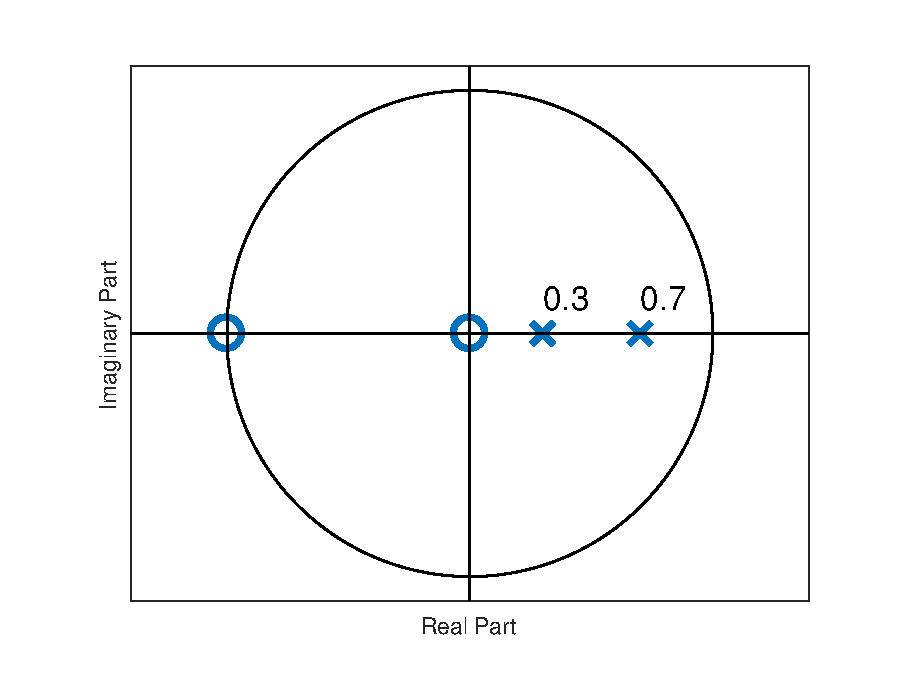
\includegraphics[width=60mm]{Q6_1.eps}
$|z|>0.7$
}
{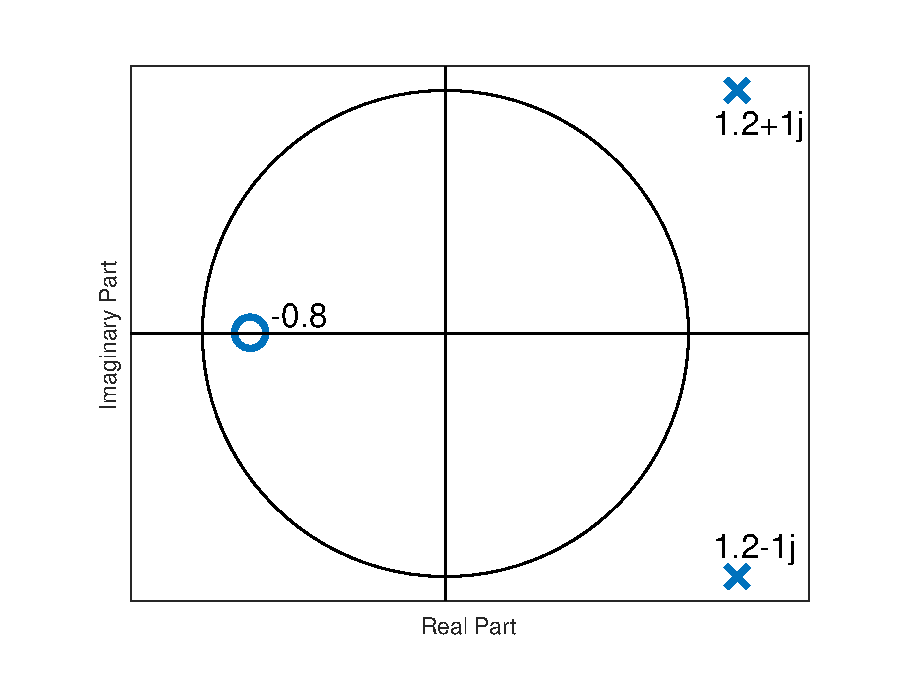
\includegraphics[width=60mm]{Q6_2.eps}
$|z|>2.44$
}
{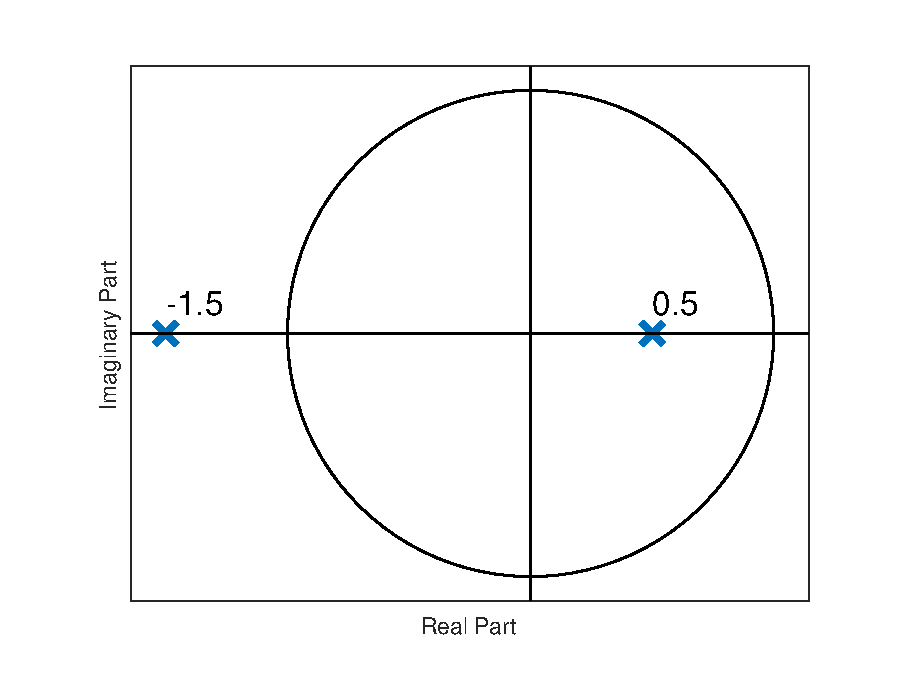
\includegraphics[width=60mm]{Q6_3.eps}
$0.5<|z|<1.5$
}
{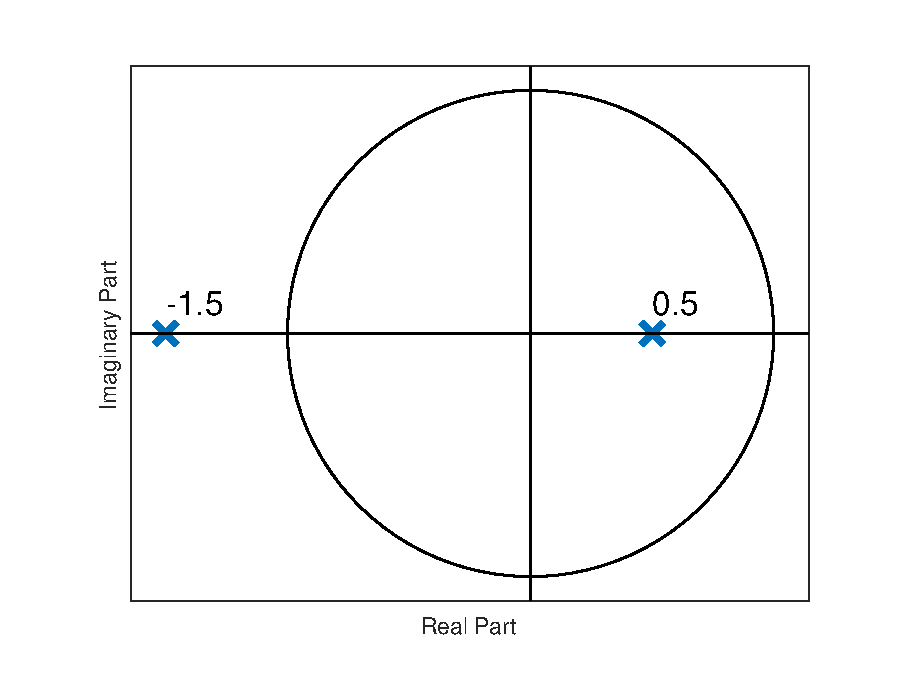
\includegraphics[width=60mm]{Q6_3.eps}
$|z|<0.5$
}
%%%%%%%%%%%%%%%%%%%%%%
\test{
اطلاعات زیر در مورد یک سیستم زمان-گسسته با ورودی $x[n]$ و خروجی $y[n]$ داده شده است:
\begin{enumerate}
\item
پاسخ این سیستم به ورودی 
$
x[n]=3^n
$
 برابر صفر است.
\item
اگر ورودی 
$
x[n]=\left({1\over 4}\right)^nu[n]
$
 به این سیستم اعمال شود، خروجی 
$$
y[n]=5\delta[n]-a\cdot\left({1\over 4}\right)^nu[n]
$$
 نتیجه خواهد شد که $a$ یک ثابت است.
\end{enumerate}
مقدار $a$ چقدر است؟
}
{$-{55\over 12}$}
{$-{29\over 16}$}
{${55\over 12}$}
{${29\over 16}$}
%%%%%%%%%%%%%%%%%%%%%%%%%%%
%\test{
%اگر تابع تبدیل یک سیستم پایدار زمان پیوسته به صورت 
%$
%H(s)={s^2+1\over s+1}
%$
% باشد، کدام گزینه به طور تقریبی، اندازه پاسخ فرکانسی این سیستم را نشان می دهد؟
%}
%{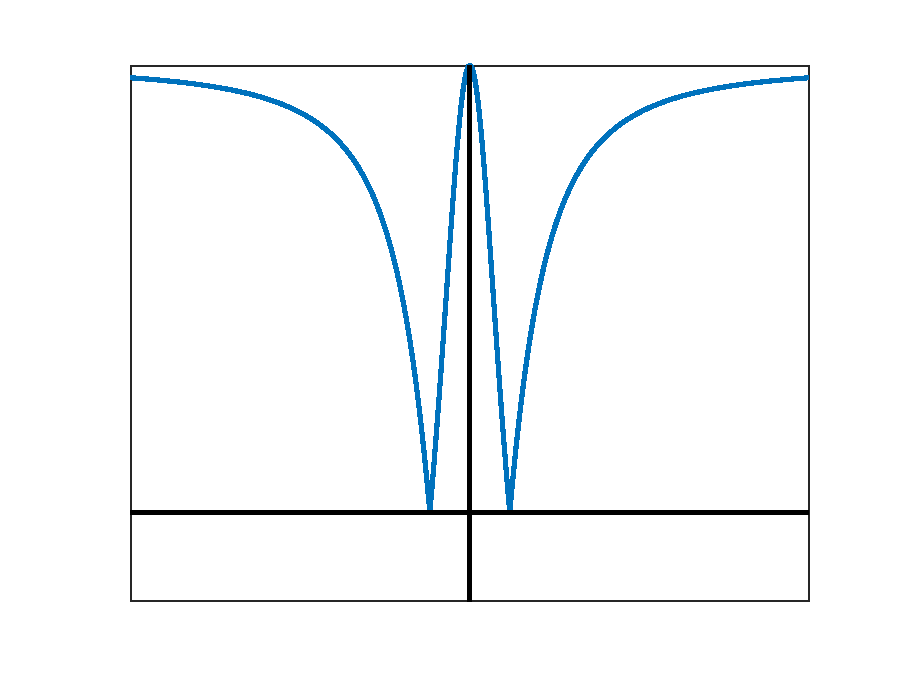
\includegraphics[width=60mm]{_Q7_1.eps}}
%{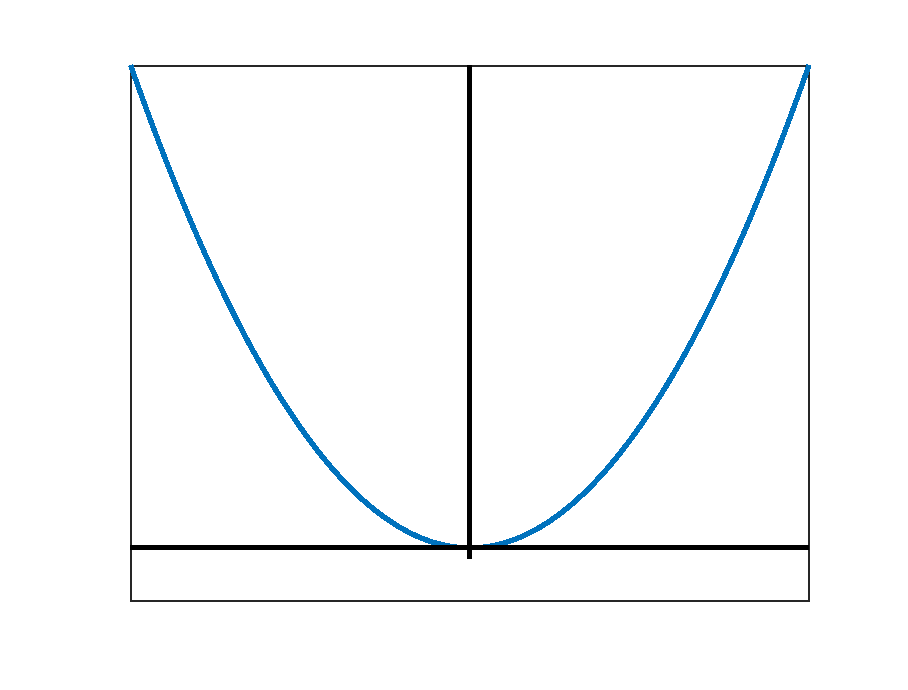
\includegraphics[width=60mm]{_Q7_3.eps}}
%{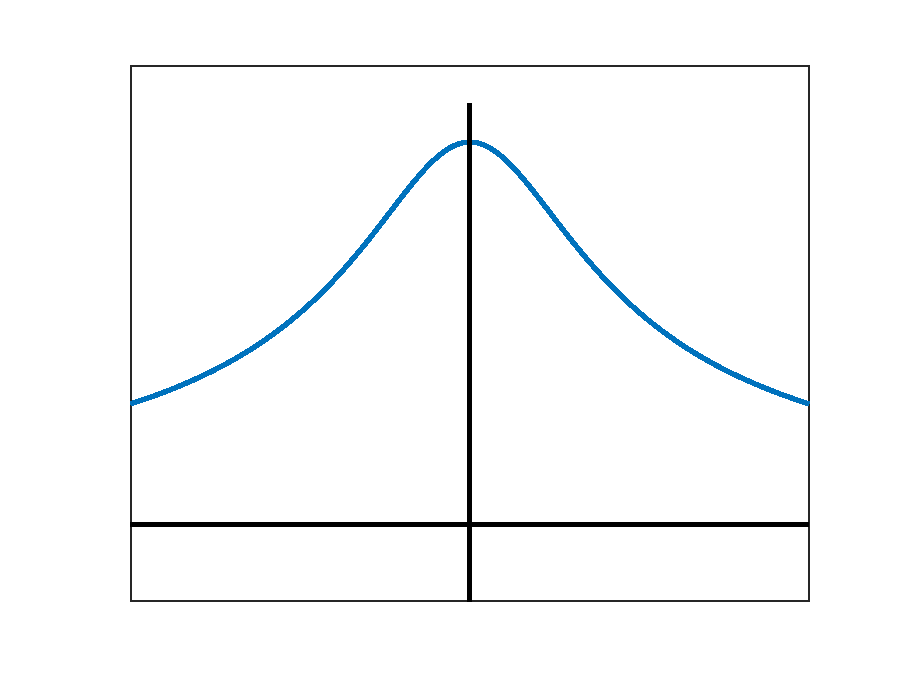
\includegraphics[width=60mm]{_Q7_2.eps}}
%{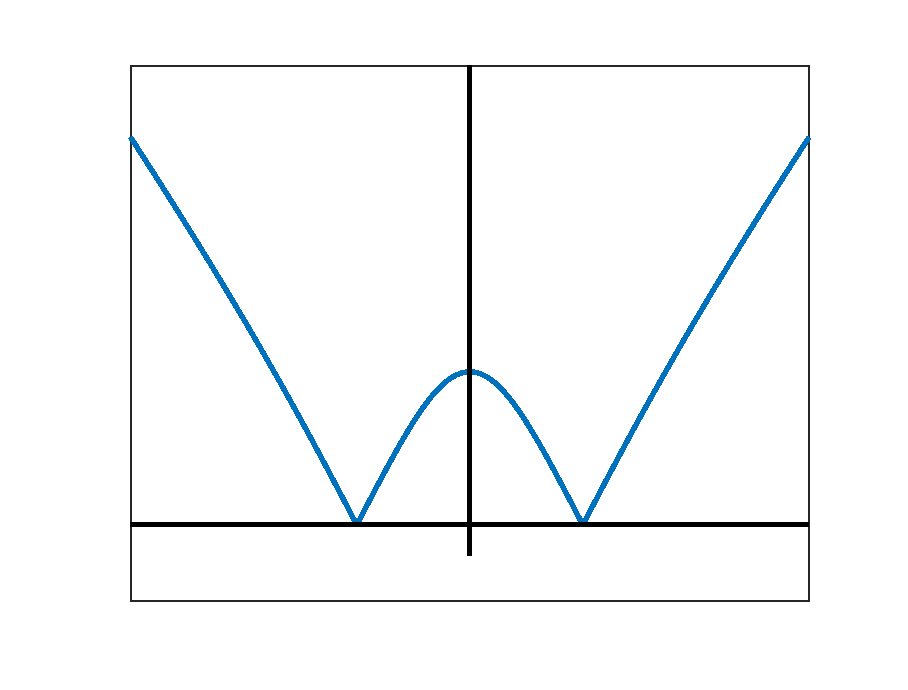
\includegraphics[width=60mm]{_Q7_4.eps}}
%%%%%%%%%%%%%%%%%%%%%%%
\test{
رابطه‌ی تبدیل لاپلاس های ورودی و خروجی یک سیستم زمان-پیوسته به صورت زیر است:
$$
Y(s)=2X^*(s^*)-{d\over ds}X(s)+5{X(s)\over s}
$$
کدام گزینه در خصوص خواص این سیستم درست است؟
}
{خطی است.}
{پایدار است.}
{مستقل از زمان است.}
{علی است.}
%%%%%%%%%%%%%%%%%%%%%%%%%%%%%%%%
\test{
رابطه‌ی تبدیل z های ورودی و خروجی یک سیستم زمان-گسسته به صورت زیر است:
$$
Y(z)=(1-z^{-1})X(z)+x[-1]
$$
کدام گزینه در خصوص خواص این سیستم درست است؟
}
{علی است.}
{مستقل از زمان است.}
{خطی است.}
{ناپایدار است.}
%%%%%%%%%%%%%%%%%%%%%%%%%%%%%%%%
\section{پرسش های تشریحی}
\Q

به سیستم علی و پایداری با تابع تبدیل
$
H(z)={1\over \left(1-{1\over 2}z^{-1}\right)^2\left(1-{1\over 3}z^{-1}\right)}
$
، ورودی 
$
x[n]=u[-n-1]
$
 اعمال می شود. در این صورت، خروجی سیستم را بیابید.
%%%%%%%%%%%%%%%

\Q

اطلاعات زیر در خصوص یک سیستم LTI زمان گسسته با پاسخ ضربه‌ی $h[n]$ و پاسخ فرکانسی 
$
H(z)
$
داده شده است.
\begin{enumerate}
\item
$h[n]$
حقیقی و دست راستی است.
\item
$
\lim_{z\to\infty}H(z)=1
$
\item
$H(z)$
دارای دو صفر است.
\item
یکی از قطب های $H(z)$ غیرحقیقی و روی دایره‌ی 
$
|z|={3\over 4}
$
 قرار دارد.
\end{enumerate}
 در این صورت:

الف) آیا این سیستم پایدار است؟ چرا؟

ب) آیا این سیستم علی است؟ چرا؟
%%%%%%%%%%%%%%%%%%

\Q

فرض کنید اطلاعات زیر، در مورد سیگنال $x(t)$ با تبدیل لاپلاس $X(s)$ داده شده است:
\begin{enumerate}
\item
$x(t)$
حقیقی و زوج است.
\item
$X(s)$
4 قطب دارد و هیچ صفر محدودی ندارد.
\item
$X(s)$
در 
$
{1\over 2}e^{j{\pi\over 4}}
$
 یک قطب دارد.
\item
$
\int_{-\infty}^{\infty} x(t)dt=4
$
\end{enumerate}
در این صورت، 
$
X(s)
$
 و ناحیه همگرایی آن را تعیین کنید.
%%%%%%%%%%%%%%%%%%%%%%%%%%
%
%\Q
%
%یک سیستم پایدار و علی دارای رابطه‌ی ورودی-خروجی زیر است:
%$$
%{d^2y(t)\over dt^2}+3{dy(t)\over dt}+2y(t)={dx(t)\over dt}-3x(t)
%$$
%(سیستم در شرایط اولیه صفر قرار دارد) در این صورت برای وارون پایدار این سیستم، پاسخ ضربه را به دست آورید.
\end{document}